% This is samplepaper.tex, a sample chapter demonstrating the
% LLNCS macro package for Springer Computer Science proceedings;
% Version 2.21 of 2022/01/12
%
\documentclass[runningheads]{llncs}
%
\usepackage[T1]{fontenc}
% T1 fonts will be used to generate the final print and online PDFs,
% so please use T1 fonts in your manuscript whenever possible.
% Other font encondings may result in incorrect characters.
%
\usepackage{graphicx}
\usepackage{listings}
\usepackage{minted}
\usepackage{hyperref}

% Used for displaying a sample figure. If possible, figure files should
% be included in EPS format.
%
% If you use the hyperref package, please uncomment the following two lines
% to display URLs in blue roman font according to Springer's eBook style:
%\usepackage{color}
%\renewcommand\UrlFont{\color{blue}\rmfamily}
%
\begin{document}
\lstset{language=haskell}
%
\title{Alternative Methods for Retaining
    Explicit and Finding Implicit Sharing in Embedded DSLs}
%
\titlerunning{Alternative Explicit and Implicit Sharing}
% If the paper title is too long for the running head, you can set
% an abbreviated paper title here
%
\author{Curtis D'Alves \and
Lucas Dutton \and
Steven Gonder \and
Christopher Kumar Anand
}
%
\authorrunning{C. D'Alves et al.}
% First names are abbreviated in the running head.
% If there are more than two authors, 'et al.' is used.
%
\institute{McMaster University, 1280 Main St W Hamilton, Canada}
%
\maketitle              % typeset the header of the contribution
%
\begin{abstract}
  Detection of sharing is a known challenge for implementers of embedded domain
  specific languages (DSLs). There are many solutions, each with their
  advantages and drawbacks. Many solutions are based on observable sharing, that
  requires either a monadic interface or use of unsafe referencing, e.g.,
  Data.Reify. Monadic interfaces are considered unsuitable for domain experts, and
  the use of unsafe referencing leads to fragile software.

  Kiselyov's methods for implicit and explicit sharing detection for finally
  tagless style DSLs is an elegant solution without having to resort to unsafe
  observable sharing. However these methods are not applicable to all types of
  DSLs (including those generating hypergraphs). We will present alternative
  methods which handle these cases. The main difference comes from the use of a
  trie to perform hash-consing. Our method for implicit sharing essentially
  trades worst-case exponential growth in computation for increased memory
  footprint. To mitigate this issue, our method for explicit sharing reduces the
  memory footprint.

\keywords{DSL  \and sharing \and common-subexpression elimination \and Haskell.}
\end{abstract}
%
%
%
\section{Introduction}

Embedded DSL's have proven useful for many applications, and there are multiple
ways of doing the embedding. Domain experts are more comfortable with embeddings
presented as a collection of pure functions. On the other hand, optimizing code
generators and other downstream uses would be much easier to implement in the
context of a monad. In particular code graph generation outside of a monad does
not benefit from observable sharing in Haskell. Kiselyov \cite{kiselyov:sharing}
solves this problem by presenting a method for implementing eDSLs in finally
tagless form that generates a directed acyclic graph (DAG) with sharing.
However, as we will explain in sections~\ref{limithashcons} and
\ref{limitexplicit}, for DSL functions that return multiple outputs (e.g.,
tuples, lists, etc.), Kiselyov's method of implicitly detecting sharing may
require computation exponential in the size of the program, and his method of
explicitly declaring sharing is inapplicable.

In the toy example
\begin{minted}{haskell}
class Exp repr where
  variable :: String -> repr Int
  constant :: String -> repr Int
  add :: repr Int -> repr Int -> repr Int
  novel :: (repr Int,repr Int) -> (repr Int,repr Int)
\end{minted}
the function \mintinline{haskell}{novel} will exhibit this issue. Since it
returns multiple outputs via a native tuple or list, it will diverge state used
to generate the DAG that cannot be captured by Kiselyov's explicit sharing
method. We will illustrate this implementation issue in Section
\ref{limitexplicit}. In our work, this translated into the inability to process
large library functions.

\smallskip
In this paper, we review Kiselyov's methods, identifying the core issue, and
present methods for implementing embedded DSLs with sharing that avoid  unsafe referencing (i.e., \mintinline{haskell}{unsafePerformIO}) \cite{gill:observablesharing}, maintain all the benefits of being embedded in the Haskell ecosystem and are computationally feasible. This
means DSL functions are pure, type-safe and can return Haskell container types (i.e.,
tuples, lists, etc.) without breaking sharing. All code will be hosted at \url{https://github.com/dalvescb/AltSharingInEDSL_Paper}

\section{Background: Detecting Sharing}

Consider the naive DSL implemented as a Haskell data type:
\begin{minted}{haskell}
data Exp
  = Add Exp Exp
  | Variable String
  | Constant Int
\end{minted}
Expressions generate Abstract Syntax Trees (ASTs),
but consider this example,
\begin{minted}{haskell}
v0 = Variable "v0"
exp0 = Add v0 (Constant 0)
exp1 = Add exp0 exp0
\end{minted}
in which the expression  \mintinline{haskell}{exp0} is shared,
and will therefore be stored once in memory.
For large expressions with lots of sharing,
this can make a substantial difference.

One of the first things the developer will do is write a pretty printer.
That recursive function will traverse the data structure as a tree,
and pretty print \mintinline{haskell}{exp0} twice.
This inefficiency is a real problem for code generation,
and naive traversal of the AST does the opposite of the common-subexpression elimination performed by a good optimizing compiler.
To avoid this,
rather than representing the code as an AST, 
we should use a DAG, retaining all of the sharing in the original DSL code. 

One way of maintaining sharing is by observable sharing (see Section 3 in \cite{kiselyov:sharing}).
In Haskell, this requires a monadic interface.
Monads are useful, but don't match the expectations of domain experts \cite{odonnell:embedding}.

\subsection{Finally Tagless DSLs}

 It would be nice
to make use of monadic state when we need it (i.e., for converting to a DAG)
while hiding it behind a nice pure interface. The finally tagless approach
\cite{carette:finallytagless} is popular for accomplishing this. In this
approach, DSL expressions are built using type-class methods that wrap the DSL in
a parameterized representation. For example, the previous data-type-based DSL
could be written in finally tagless style as

\begin{minted}{haskell}
class Exp repr where
  add :: repr Int -> repr Int -> repr Int
  variable :: String -> repr Int
  constant :: Int -> repr Int
\end{minted}

We can then create different instances to implement different functionality.
For example, we can implement a pretty printer
\begin{minted}{haskell}
newtype Pretty a = Pretty { runPretty :: String }

instance Exp Pretty where
  add x y = Pretty $ "("++runPretty x++") + ("++runPretty y++")"
  variable x = Pretty x
  constant x = Pretty $ show x
\end{minted}

Or generate an AST
\begin{minted}{haskell}
newtype AST a = AST { genAST :: Exp }

instance Exp AST where
  add x y =  AST $ Add (genAST x) (genAST y)
  variable x = AST $ Variable x
  constant x = AST $ Constant x
\end{minted}

Finally tagless style provides extensible, user friendly DSLs.

\subsection{Implicit Sharing via Hash-Consing}

The goal of detecting sharing is to generate a graph structure (like the AST in
the previous section) that share's common subexpressions. So we're essentially
going to generate a Directed Acyclic Graph (DAG) instead of an AST. For example,
we can use the following DAG structure that explicitly references nodes by a
unique identifier

\begin{minted}{haskell}
type NodeID = Int
data Node = NAdd NodeID NodeID
          | NVariable String
          | NConstant Int

newtype DAG = DAG (BiMap Node) deriving Show
\end{minted}

Kiselyov's method for detecting implicit sharing in finally tagless style uses
hash-consing \cite{kiselyov:sharing}. Hash-consing is based on a bijection of
nodes and a set of identifiers, e.g.,

\begin{minted}{haskell}
data BiMap a -- abstract
lookup_key :: Ord a => a -> BiMap a -> Maybe Int
lookup_val :: Int -> BiMap a -> a
insert :: Ord a => a -> BiMap a -> (Int,BiMap a)
empty :: BiMap a
\end{minted}

The method can be performed using any data structure that provides the above
interface. An efficient implementation would use hashing and linear probing, as
is done by Thai in his Master's thesis \cite{thai2021type}.

In order to generate such a data structure, we will need to keep track of the
current maximum identifier to keep them unique. The representation for the
finally tagless instance is then a wrapper around a state monad that holds the
DAG being constructed in its state and returns the current (top)
\mintinline{haskell}{NodeID}:

\begin{minted}{haskell}
newtype Graph a = Graph { unGraph :: State DAG NodeID }

instance Exp Graph where
  constant x = Graph (hashcons $ NConstant x)
  variable x = Graph (hashcons $ NVariable x)
  add e1 e2 = Graph (do
                     h1 <- unGraph e1
                     h2 <- unGraph e2
                     hashcons $ NAdd h1 h2)
\end{minted}

The trick to uncovering sharing is in the
\mintinline{haskell}{hashcons} function, which inserts a new node into the current DAG, but not
before checking if it is already there.
\begin{minted}{haskell}
hashcons :: Node -> State DAG NodeID
hashcons e = do
  DAG m <- get
  case lookup_key e m of
    Nothing -> let (k,m') = insert e m
               in put (DAG m') >> return k
    Just k -> return k
\end{minted}

The technique is essentially that of hash-consing, popularized by its use in
LISP compilers, but discovered by Ershov in 1958 \cite{ershov1958:consing}.
Other works have explored the use of type-safe hash-consing in embedded DSLs,
see \cite{filliatre:typesafeconsing}.

\subsection{Limitations of Hash-Consing} \label{limithashcons}

When we wrap our state monad in finally tagless style, we lose some expected
sharing. In the following code, the use of the let causes the computation
$x + y$ to only occur once
\begin{minted}{haskell}
haskellSharing x y =
 let
   z = x + y
 in z + z
\end{minted}

Implicit sharing via hash-consing prevents duplication in the resulting DAG, but
unfortunately doesn't prevent redundant computation. Consider the following
equivalent attempt at using Haskell's built-in sharing in the finally tagless DSL
\begin{minted}{haskell}
dslSharing :: Exp Graph -> Exp Graph -> Exp Graph
dslSharing x y =
  let
    z = add x y
  in add z z
\end{minted}
Knowing that \mintinline{haskell}{z} is a wrapper around a state monad,
and recalling the implementation of
\mintinline{haskell}{add} via hash-consing above, 
the values \mintinline{haskell}{h1} and \mintinline{haskell}{h2} are
separately evaluated through the state monad, even if \mintinline{haskell}{e1} and \mintinline{haskell}{e2} are the same shared Haskell value. 
Hash-consing will prevent these redundancies from appearing in
the resulting DAG, 
but in the process of discovering the sharing, the entire unshared AST will still be traversed.

Consider a chain of \mintinline{haskell}{add}s  with sharing, for example
\begin{minted}{haskell}
addChains :: Exp repr => Expr Int -> Expr Int
addChains x0 = 
  let
    x1 = add x0 x0
    x2 = add x1 x1
    ...
  in xn
\end{minted}

\vspace{-1cm}
\begin{figure}
  \centering
  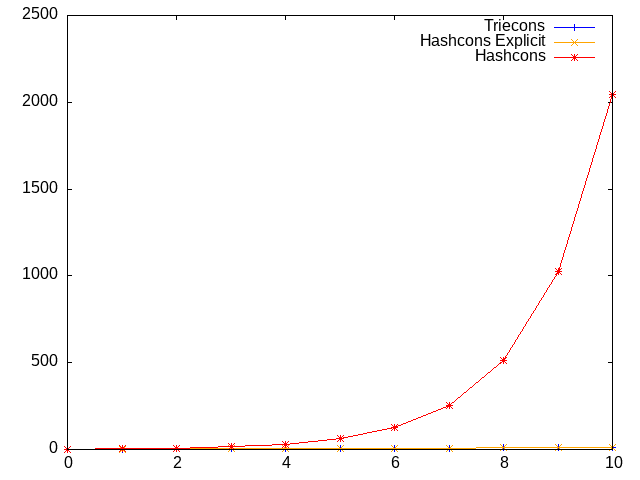
\includegraphics[width=0.6\textwidth]{figs/hashconscmp.png}
  \caption{Number of calls to \mintinline{haskell}{hashcons} plotted against the
    number of \mintinline{haskell}{add} operations performed.
    Hash-consing is performed without explicit sharing and is clearly exponential,
    Triecons (without explicit sharing) and Hashcons Explicit (with explicit
    sharing) overlap and are both linear
  } \label{fig:hashcons}
\end{figure}
As shown in Fig.~\ref{fig:hashcons}, this code will perform approximately
$2^{n+1}$ \mintinline{haskell}{hashcons} operations, where $n$ is the number of \mintinline{haskell}{add}s.

\subsection{Explicit Sharing and Limitations} \label{limitexplicit}

Kiselyov \cite{kiselyov:sharing} recognized that the amount of computation with
hash-consing ``may take a long time for large programs,'' and proposed an ad-hoc
solution, explicit sharing via a custom let construct
\begin{minted}{haskell}
class ExpLet repr where
  let_ :: repr a -> (repr a -> repr b) -> repr b
instance ExpLet Graph where
  let_ e f = Graph (do x <- unGraph e
                     unGraph $ f (Graph (return x)))
\end{minted}
which can be used to rewrite \mintinline{haskell}{addChains} as
\begin{minted}{haskell}
addChains x =
  let_ x (\x0 ->
  let_ (add x0 x0)  (\x1 ->
  let_ (add x1 x1)  (\x2 ->
   ...
  )))
\end{minted}
This makes the code a bit clunky and adds an extra burden on the DSL writer, but
it prevents unnecessary hash-consing in our example.

However the method does not work for DSL functions returning multiple outputs
via tuples or container types like lists. If we're attempting to generate a more
specific graph structure like a hypergraph or bi-partite graph the need to do
this becomes more aparent. For example, in our own research we implemented a DSL
for an instruction set architecture that generates a bipartite graph of
instructions and the registers they act upon. Attempting to generate a graph
where an instruction outputs multiple registers will result in returning
multiple independent state monads.

We can more concisely illustrate this problem by adding the following
instruction to our DSL that attempts to return two separate nodes in the DAG at
once
\begin{minted}{haskell}
novel :: (repr Int,repr Int) -> (repr Int,repr Int)
\end{minted}

The issue is that DAG generation requires splitting the state monad in two:
\begin{minted}{haskell}
instance Exp Graph where
  ...
  novel e1 e2 = let
     g1 = Graph (do h1 <- unGraph e1
                    h2 <- unGraph e2
                    hashcons $ Novel1 h1 h2)
     g2 = Graph (do h1 <- unGraph e1
                    h2 <- unGraph e2
                    hashcons $ Novel2 h1 h2)
     in (g1,g2)
\end{minted}
Each output it returns will now have to be individually evaluated, so a chain of
DSL functions that output 2 or more values will suffer from the same exponential
explosion of hash-consing operations, and trying to adapt the let construct above,
just creates another function with the same problem (multiple outputs).

One solution to this issue is to integrate container types such as tuples and
lists into the DSL language. However doing this eliminates the advantage of
having an embedded language. Manipulating tuple values will be cumbersome,
constantly requiring calls to custom implementations of
\mintinline{haskell}{fst}, \mintinline{haskell}{snd} etc. And for lists you'll
lose access to built-in Haskell list functionality.

\section{Implicit Sharing Via Byte String ASTs}

The heart of our problem is that whenever we need to sequence the state of the inputs
for one of our DSL functions we want to first check if it's already been
evaluated. But how do we do that without first evaluating it to gain access to
its unique identifier? We need some way to uniquely identify it outside the monad.

Our proposed solution is to build a serialized AST using byte strings for each node along with our
DAG.
The byte string stays outside the monad, while the DAG remains inside.
We can do this efficiently by replacing the \mintinline{haskell}{BiMap}
with a trie.
In our toy example, we use the package \texttt{bytestring-trie}.
% TODO reference literature on tries

\begin{minted}{haskell}
data Graph a = Graph { unGraph :: State DAG NodeID
                     , stringAST :: ByteString }

data DAG = DAG { unTrie :: Trie (Node,NodeID)
               , maxID  :: NodeID
               } deriving Show
\end{minted}
This looks a bit different because the \mintinline{haskell}{BiMap}
was a bijective relation between nodes and node ids,
whereas the trie maps byte strings to pairs (node,node id).
To get the DAG expressed as a relation, project out the values of the trie.

To prevent confusion, we name the hash-consing function in our method \mintinline{haskell}{triecons}:
\begin{minted}{haskell}
triecons :: ByteString -> Node -> State DAG NodeID
triecons sAST node = do
  DAG trie maxID <- get
  case Trie.lookup sAST trie of
    Nothing -> let maxID' = maxID+1
                   trie' = Trie.insert sAST (node,maxID') trie
                in do put $ DAG trie' maxID'
                      return maxID'
    Just (_,nodeID) -> return nodeID
\end{minted}
We use it to implement the DAG-building instance of the DSL,
which looks a lot like the previous instance.
The substantial differences are the 
\mintinline{haskell}{buildStringAST} calls
which you can think of as pretty printing, but optimized for the trie,
and the use of \mintinline{haskell}{seqArgs} (explained below):
\begin{minted}{haskell}
instance Exp Graph where
  constant x = let
    node = NConstant x
    sAST = buildStringAST node []
    in Graph (triecons sAST $ NConstant x) sAST
  variable x = let
    node = NVariable x
    sAST = buildStringAST node []
    in Graph (triecons sAST $ NVariable x) sAST
  add e1 e2 = let
      sAST = buildStringAST "nadd" [e1,e2]
      sT = do ns <- seqArgs [e1,e2]
              case ns of
                [n1,n2] -> triecons sAST $ NAdd n1 n2
                _ -> error "black magic"
    in Graph sT sAST
\end{minted}
The magic is in \mintinline{haskell}{seqArgs}.
We only evaluate the inner state \mintinline{haskell}{sT} of each argument if we
fail to find its corresponding serialized AST in the Trie.
\begin{minted}{haskell}
seqArgs :: [Graph a] -> State DAG [NodeID]
seqArgs inps =
  let
    seqArg (Graph sT sAST) =
      do DAG trie _ <- get
         case Trie.lookup sAST  trie of
           Nothing -> sT
           Just (_,nodeID) -> return nodeID
  in sequence $ map seqArg inps
\end{minted}

This will prevent
redundant hash-consing without the need for explicit sharing,
but at the expense of storing redundant byte strings. 

\subsection{Memory Limitations}
The byte string AST being built will itself suffer from lack of sharing. We're
essentially trading extra computation for extra memory. In our 
\mintinline{haskell}{addChains} example from Section~\ref{limithashcons}, our
method now has exponential scaling in memory instead of computation. This can be
a good tradeoff, since memory is so plentiful in modern hardware, but still
presents an issue.

\section{Explicit Sharing Of ByteString ASTs}
We propose another solution to this issue, taking inspiration again from Kiselyov  
\cite{kiselyov:sharing}, by introducing an explicit construct for specifying
sharing. This time, the construct will substitute the current byte string for a
more compact label.

\begin{minted}{haskell}
class Substitute repr where
  subT :: ByteString -> repr a -> repr a
instance Substitute Graph where
  subT s' (Graph g s _) = Graph g s' (Just s)

exampleSubT x y = let
  z = subT "z" (add x y)
  in add z z
\end{minted}

For safety purposes, we need to keep track of a table of these labels and their
corresponding ASTs, to make sure we don't use the same label for different ASTs.
\begin{minted}{haskell}
data DAG = DAG { dagTrie :: Trie (Node,NodeID)
               , dagSubMap :: Map ByteString ByteString
               , dagMaxID :: Int
               } deriving Show

data Graph a = Graph { unGraph :: State DAG NodeID
                     , unStringAST :: ByteString
                     , unSubT :: Maybe ByteString }
\end{minted}

When a substitution is made via \mintinline{haskell}{subT}, the
\mintinline{haskell}{unStringAST} field is replaced with the new label, and the
previous serialized AST is placed in \mintinline{haskell}{unSubT}. When a
\mintinline{haskell}{Graph} value is processed, the \mintinline{haskell}{unSubT}
field is checked for if it contains a label

\begin{minted}{haskell}
seqArgs :: [Graph a] -> State DAG [NodeID]
seqArgs inps =
  let
    seqArg (Graph sT sAST mSubt) =
      do DAG trie _ _ <- get
         let sAST' = case mSubt of
                       Just s -> s
                       Nothing -> sAST
         case Trie.lookup sAST' trie of
           Nothing -> sT -- error "missing ast"
           Just (node,nodeID) ->
              do subTInsert mSubt sAST (node,nodeID)
                 return nodeID
  in sequence $ map seqArg inps
\end{minted}

If the \mintinline{haskell}{unSubT} field contains a label, that means the
current \mintinline{haskell}{unStringAST} field is a substitution that needs to
be inserted into \mintinline{haskell}{dagSubMap}. The function
\mintinline{haskell}{subTInsert} handles this

\begin{minted}{haskell}
subTInsert :: Maybe ByteString -> ByteString
           -> (Node, NodeID) -> State DAG ()
subTInsert Nothing  _ _  = return ()
subTInsert (Just s) sAST nodeID =
  do DAG trie subtMap _ <- get
     case Map.lookup sAST subtMap of
        Just sAST' -> if sAST == sAST'
                      then return ()
                      else error "tried to resubT"
        Nothing -> let cMap' = Map.insert sAST s subtMap
                       trie' = Trie.insert sAST nodeID trie
                  in modify (\dag -> dag { dagTrie = trie'
                                      , dagSubMap = cMap' })
\end{minted}

We need to make sure we don't attempt to insert the same substitution for two
different ASTs. Unfortunately, if there is a collision there's no way to escape
the state monad to prevent or modify the substitution. In the toy example,
compilation crashes, but we could catch an exception instead. Either way it's up
to the DSL writer to ensure they don't reuse the same label as a substitution.

\section{BenchMarking}

Even with explicit sharing via substitutions, our method contains a reasonable
amount of overhead in order to overcome the shortcomings of Kiselyov's method.
The \mintinline{haskell}{addChains} example altered for explicit sharing with
both methods presents a worst case scenario in terms of overhead comparison.
Kiselyov's method is able to fully utilize its explicit sharing and our method
requires many substitution lookups.

\begin{table}
  \begin{tabular}{|l|l|l|l|l|l|l|l|}
    \hline
    {\bf Size } &  150 & 200 & 10000 & 50000 \\
    \hline
    {\bf Hash-Cons time } &  0.0 secs & 0.0 secs & 0.01 secs & 0.03 secs \\
    {\bf Hash-Cons alloc } &  619,296 bytes & 739,304 bytes & 28,662,592 bytes & 155,993,544 bytes \\
    {\bf Trie-Cons time } &   0.0 secs & 0.0 secs & 0.03 secs & 0.16 secs \\
    {\bf Trie-Cons alloc } &  1,773,416 bytes & 2,333,680 bytes & 129,146,808 bytes & 723,437,504 bytes \\
    \hline
  \end{tabular}

  \vspace{1mm}
  \caption{Benchmarks of \mintinline{haskell}{addChains} example with full
    explicit sharing.}\label{tab1}
\end{table}

Table \ref{tab1} gives a set of benchmarks comparing our method with Kiselyov's,
both taking full advantage of explicit sharing. It's clear Kiselyov's method
performs better in this situation, however it should be noted our method is
still viable for solving very large DAG's in reasonable amounts of time / memory.

For more interesting benchmarks, we need to consider a more sophisticated DSL.
We can define a DSL for an instruction set architecture like mentioned in
section \ref{limitexplicit}. It will have the following interface

\begin{minted}{haskell}
class ISA repr where
  -- | Load from memory into a GPR
  ldMR :: repr MR -> Int -> (repr GPR, repr MR)
  -- | Store a GPR into memory
  stdMR   :: repr MR -> Int -> repr GPR -> repr MR
  -- | Bitwise NAND of two 64-bit general-purpose registers (NNGRK)
  nandG   :: repr GPR -> repr GPR -> repr GPR
  -- | Bitwise NOR of two 64-bit general-purpose registers (NOGRK)
  norG    :: repr GPR -> repr GPR -> repr GPR
  -- | Bitwise NXOR of two 64-bit general-purpose registers (NXGRK)
  eqvG    :: repr GPR -> repr GPR -> repr GPR
  -- | Addition of two 64-bit general-purpose registers (AGRK)
  addG    :: repr GPR -> repr GPR -> repr GPR
  ...
\end{minted}

This language can be used to encode basic blocks of assembly code. These basic
blocks may return multiple outputs, preventing us from using explicit sharing
via let constructs. For example,
\begin{minted}{haskell}
add2 :: ISA repr => (repr GPR, repr GPR) -> (repr GPR, repr GPR)
add2 (a, b) =
    let
        a' = addG a b
        b' = addG a' b
    in (a', b')
\end{minted}

We used this language to implement approximations of vector
\mintinline{haskell}{cos} and \mintinline{haskell}{tan} (i.e., a loop body that
computes over an input and output array). The loop body was unrolled by a factor
of four making for a sufficiently large resulting DAG.

We profiled \mintinline{haskell}{cos} using both Kiselyov's method (i.e., hash-consing) and are own
(i.e., trie-consing with some explicit sharing). It wasn't possible to use
Kiselyov's explicit sharing method where meaningful so our code was able to
achieve greater performance, with only a small increase in memory consumption
(see Fig.~\ref{fig:hashvscons}).

\begin{figure}[!h]
  \centering
  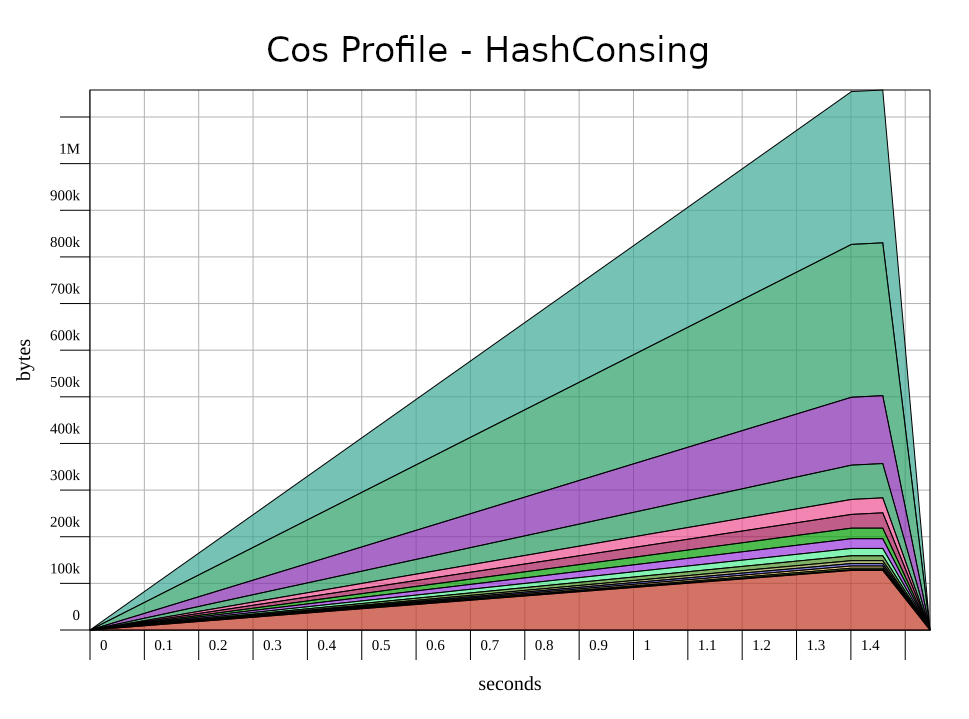
\includegraphics[width=0.6\textwidth]{figs/cos_profile_hashcons_cropped.png}
  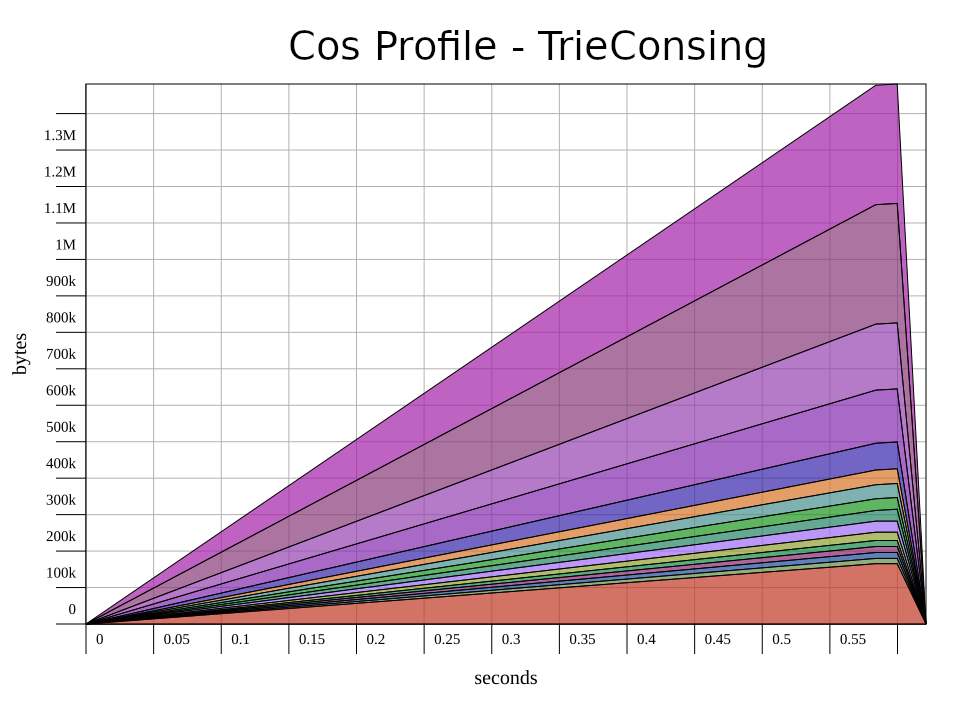
\includegraphics[width=0.6\textwidth]{figs/cos_profile_triecons_cropped.png}
  \caption{Comparison of cos using hash-cons vs trie-cons}
  \label{fig:hashvscons}
\end{figure}


For \mintinline{haskell}{tan}, we were unable to generate a resulting code graph using Kiselyov's
method. Using explicit sharing via let constructs wasn't possible due to the
multiple outputs issue and without it the amount of computation due to redundant
hash-consing was simply too large to perform in a reasonable amount of time.

We were able to generate \mintinline{haskell}{tan} using our method both without and with our explicit
sharing, however without explicit sharing we consumed an unreasonable amount of
memory (see Fig.~\ref{fig:explicitvsno}). It should be noted, the main source of
redundant computation in \mintinline{haskell}{tan} is the reuse of computed values of
\mintinline{haskell}{cos} and \mintinline{haskell}{sin}. By simply explicitly
sharing just those values we achieved the significant speedup shown in
Fig.~\ref{fig:explicitvsno}.

\begin{figure}[!h]
  \centering
  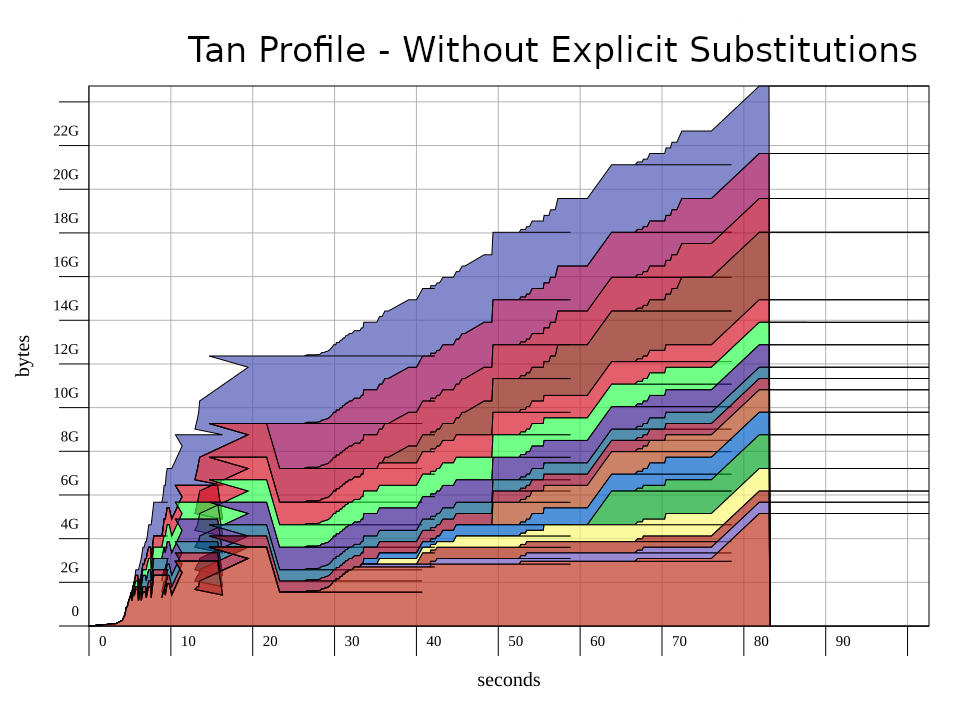
\includegraphics[width=0.6\textwidth]{figs/noexplicit_cropped.png}
  \hfill
  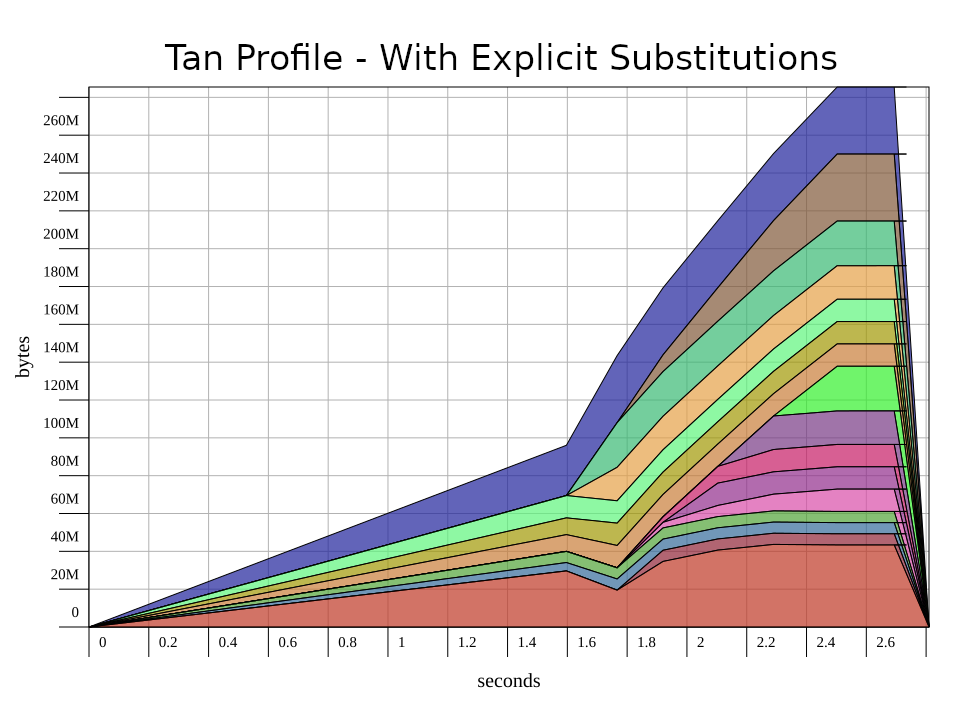
\includegraphics[width=0.6\textwidth]{figs/explicit_cropped.png}
  \caption{Comparison of tan profiling using no explicit sharing vs explicit}
  \label{fig:explicitvsno}
\end{figure}

\section{Conclusion and Future Work}
We have presented a method for constructing finally tagless style DSLs with
sharing detection, that allows for DSLs specifying hypergraphs (e.g., functions
with multiple outputs). It also avoids the use of unsafe referencing as
performed when doing observable sharing, c.f. \cite{gill:observablesharing}.

The method has its drawbacks in terms of memory usage, but these can be
mitigated by explicitly specifying sharing. This does present an extra burden on
the DSL writer to implement explicit sharing when necessary and ensure labels
are not reused. Future work may investigate the use of a preprocessor or plugin
to automate explicit sharing. Unlike an explicit let construct, it would be
fairly straightforward to automatically bind \mintinline{haskell}{subT}
operations to any DSL function call.

\subsubsection{Acknowledgements} We thank NSERC and IBM Canada Advanced Studies for supporting this work.
%
% ---- Bibliography ----
%
% BibTeX users should specify bibliography style 'splncs04'.
% References will then be sorted and formatted in the correct style.
\bibliographystyle{splncs04}
\bibliography{references}

\end{document}

% LocalWords:  DSLs unsafePerformIO Haskell's AST typeclass tagless Trie
% LocalWords:  Kiselyov's haskell consing hypergraphs
% Local Variables:
% LaTeX-verbatim-environments-local: ("minted")
% eval: (setq-local LaTeX-indent-environment-list (cons '("minted" current-indentation) (default-value 'LaTeX-indent-environment-list)))
% End:
